\chapter{Tree-structure segmentation for logistic regression} \label{chap6}

\epigraph{.}{.}

\minitoc


\textit{Nota Bene :} Ce chapitre s'inspire fortement ... \textcolor{red}{à adapter au moment de l'envoi du manuscrit}

\bigskip

\selectlanguage{english}

In Chapter~\ref{chap1}, and parallel to quantization, it was argued in Section~\ref{subsec:segmentation} that, what is referred to as ``segmentation'' in the \textit{Credit Scoring} industry, could also be a straightforward solution to deal with missing values and outliers. The more theoretical justification of quantization, sketched in Section~\ref{sec:bias_variance_quant}, was to achieve a good bias-variance tradeoff of the predictive task. This goal was embedded in the proposed quantization algorithm. Here again, the resulting segmentation and scorecards therein can be viewed as a single model for the whole population. In the next Section, the industrial context of the problem is set, which is followed in Section~\ref{sec:literature} by a literature review. Section~\ref{sec:model_selec_tree} reinterprets this problem, as promised, as a model selection problem for which a specific approach is designed in subsequent Sections.


\section{Introduction}

\subsection{Context}

As was emphasized in all previous Chapters, \gls{lr} is the building block of a scorecard predicting the creditworthiness of an applicant and partly automating the acceptance / rejection mechanism. However, estimating \gls{lr} coefficients means that training data $(\glssymbol{bbx},\glssymbol{bby})$ is available. This is not the case when a new product, \textit{e.g.}\ smartphone leasing, is added to the acceptance system. On a practical note, some other previously learnt scorecard may not be applicable on this new market because the same information is not asked to applicants, \textit{e.g.}\ marital status, because given the low amounts at stake, it was decided to collect the fewest data possible, to make the process as simple and quick as possible. On a more theoretical note, it is probable that applicants to smartphone leasing are not stemming from the same data generating mechanism $p(\glssymbol{bX},Y)$ as any other previous applicants (\textit{i.e.}\ on other markets). Put it another way, the possibility of having several \gls{lr} scorecards on sub-populations of the total portfolio allows to have more flexibility, and thus potentially reduces model bias discussed in Chapter~\ref{chap1}.

For these reasons, several industries, among which \textit{Credit Scoring}, rely on several ``weak learners'' such as \gls{lr}, arranged in a tree. It is assumed there are $K$ ``clusters'' which form the leaves of this tree and which assigning latent random feature is denoted by $C$ (lower-case for observations). The other notations employed inspire from the preceding Chapters: the superscript notation is used to insist on the fact that available features $\glssymbol{bx}^c$ differ potentially in each of the scorecards. It follows that quantizations $\q^c$ and interactions $\bdelta^c$, discussed in Chapters~\ref{chap4} and~\ref{chap5} respectively, are also different. Consequently, the \gls{lr} coefficients $\glssymbol{bth}^c$ are also obviously different.

Such decision process is illustrated on Figure~\ref{fig:arbre}. This tree structure and the vocabulary of ``weak learners'' would indicate a use-case of well-known Mixtures of Experts~\cite{jordan1994hierarchical} or aggregation / ensemble methods~\cite{opitz1999popular} respectively. However, as is covered by the~\nameref{sec:literature}, these fuzzy methods imply, among other incompatibilities that all applicants are scored by all scorecards, which is obviously neither desirable (for interpretation purposes) nor feasible (since available features differ).

The next Section illustrates how such a structure is achieved using \gls{cacf}'s in-house practices.

\tikzstyle{level 1}=[level distance=2.2cm, sibling distance=7cm]
\tikzstyle{level 2}=[level distance=2cm, sibling distance=5cm]
\tikzstyle{level 3}=[level distance=2cm, sibling distance=3cm]

\begin{figure}
\resizebox{\textwidth}{!}{
\centering
\begin{tikzpicture}
  [
    sibling distance        = 15em,
    level distance          = 5em,
    edge from parent/.style = {draw, -latex},
    every node/.style       = {font=\footnotesize},
    sloped
  ]
  \node [root] {\textcolor{black}{Applicants}}
    child { node [dummy] {}
      child { node [dummy] {}
        child { node [env] {\textcolor{black}{$p_{\glssymbol{bth}^1}(y|\q^1(\glssymbol{bx}),\bdelta^1))$\hspace*{-0.2cm}}}
          edge from parent node [below] {Renters} }
        child { node [env] {\textcolor{black}{$p_{\glssymbol{bth}^2}(y|\q^2(\glssymbol{bx}),\bdelta^2)$}}
          edge from parent node [above] {Salaried} }
        child { node [env] {\textcolor{black}{$p_{\glssymbol{bth}^3}(y|\q^3(\glssymbol{bx}),\bdelta^3)$}}
                edge from parent node [above] {Others} }
        edge from parent node [above] {Revolving} }
      child { node [env] {\textcolor{black}{$p_{\glssymbol{bth}^4}(y|\q^4(\glssymbol{bx}),\bdelta^4)$}}
              edge from parent node [above, align=center]
                {Standard loan} }
              edge from parent node [above] {Home Appliances} }
    child { node [dummy] {}
      child { node [dummy] {}
        child { node [env] {\textcolor{black}{$p_{\glssymbol{bth}^5}(y|\q^5(\glssymbol{bx}),\bdelta^5)$}}
          edge from parent node [above] {Leasing} }
        child { node [env] {\textcolor{black}{$p_{\glssymbol{bth}^6}(y|\q^6(\glssymbol{bx}),\bdelta^6)$}}
                edge from parent node [above] {Standard loan} }
        edge from parent node [above] {Fiat} }
      child { node [env] {\textcolor{black}{$p_{\glssymbol{bth}^7}(y|\q^7(\glssymbol{bx}),\bdelta^7)$}}
              edge from parent node [above, align=center]
                {Kawasaki} }
              edge from parent node [above] {Automobile} };
\end{tikzpicture}
}
\caption{Simplified cartography of the application scorecards.}
\label{fig:arbre}
\end{figure}




\subsection{In-house \textit{ad hoc} practice}

\textit{Credit Scoring} practitioners are often asked by the management to study ``locally'' the decision process displayed on Figure~\ref{fig:arbre} by \textit{e.g.}\ merging branches (for example Standard loans and Leasing for Fiat) or conversely to spread sub-populations (for example Kawasaki into Standard loans and Leasing). The same is applicable when one or several scorecards are deemed too old or a new market / product is added to the portfolio: the analyst has to detail how many scorecards have to be built and why.

To do so, the in-house practice .

\paragraph{\gls{pca}}

The goal of \gls{pca}~\cite{pages2014multiple} is to represent observations graphically in a way that exhibits most efficiently their similitude and differences by combining input features in so-called orthogonal ``principal components'' $\bm{u} = (\bm{u}_1,\dots,\bm{u}_d)$ such that the inertia $\glssymbol{x}_i' \bm{u}_j$ of each axis $j$ is maximized. It can be shown that it is equivalent to seeking the ordering of the eigenvalues $\bm{\lambda} = (\lambda_1,\dots,\lambda_d)$ of the covariance matrix $\Sigma = \glssymbol{bbx}'\glssymbol{bbx}$. The explained variance of each axis $j$ is given by $\frac{\lambda_j}{\sum_{j'=1}^d \lambda_j'}$. Classically, only the two first axes $(\bm{u}_1,\bm{u}_2)$ are used to represent graphically the data in this new space and the \textit{Credit Scoring} practitioner decide if, visually, clusters are formed (\textit{i.e.}\ clouds with little intra-class variance) which would be used to build separate scorecards $(p_{\glssymbol{bth}^{1}},p_{\glssymbol{bth}^{2}})$, as is the case on Figure~\ref{fig:pca}. The method is described in Appendix~\ref{app1:pca}.

However, the \textit{Credit Scoring} data is of mixed type and \textit{Credit Scoring} practitioners are used to quantizing the data as in Chapter~\ref{chap4} before testing for homogeneous clusters by using \textit{e.g.\ equal-freq} or $\chi^2$ tests (see Appendix~\ref{app1}).

\paragraph{\gls{mca}}

In presence of only categorical features (or following quantization), the \gls{mca} algorithm is more appropriate: it extends the \gls{pca} approach to categorical features by using the disjunctive table (dummy / one-hot encoding of $\glssymbol{bbx}$). For a thorough introduction to \gls{mca}, see \textit{e.g.}~\cite{lebart1995statistique}. What is most interesting in this method is that both categorical features' levels and observations can be simultaneously displayed on the first principal components axes, as is the case on Figure~\ref{fig:mca}. The method is described in Appendix~\ref{app1:mca}. This is of high practical interest in \textit{Credit Scoring} because clouds of points are directly characterized by the categorical levels that are displayed nearest, contrary to \gls{pca} where groups correspond to surfaces of equation $\glssymbol{bx} ' \bm{u}_1 + \glssymbol{bx} ' \bm{u}_2 \geq \alpha$ where $alpha$ encodes the separation boundary of resulting clusters, which would be the edges of our decision system, as on Figure~\ref{fig:arbre}, and make it arguably less interpretable.

Nevertheless, a method applicable to mixed data exists as well and could directly be applied to ``raw'' features.

\paragraph{\gls{famd}}

The \gls{famd} algorithm~\cite{pages2014multiple} aims at performing both \gls{mca} on categorical features and \gls{pca} on continuous features in a simultaneous fashion. Resulting principal component axes depend on both data types, as can be seen from Figure~\ref{fi:famd}. The method is described in Appendix~\ref{app1:famd}. This method has the advantage of not requiring the \textit{Credit Scoring} practitioner to preprocess the ``raw'' data by quantizing it, which could have a huge impact on the results of the subsequent method employed, as argumented in Chapter~\ref{chap4}. Moreover, the practitioner would fine-tune the quantization of each sub-population which, if fed back to the \gls{mca}, would potentially yield completely different results!

It appears clearly that all these methods do not directly optimize a predictive goal such as the one optimized by \gls{lr}. Moreover, the \textit{ad hoc} preprocessing step of quantization might influence the structure of the retained segmentation. 

For numerical experiments of Section~\ref{sec:num_exp}, the \gls{famd} approach will be used.


\subsection{These practices can fail}

Of course, like all \textit{ad hoc} methods that rely on ``two-stages'' procedures which do not share a common objective, the aforementioned in-house practice can fail. \textit{Credit Scoring} practitioners are probably aware that their methods are not bullet-proof, but like most industries, unless proven and provided to them with easily usable software, these practices remain.

This Chapter has no intent in filling that gap as was ambitioned in Chapters~\ref{chap4} and~\ref{chap5} but rather to give insights on more elaborate, readily usable methods that will be covered in Section~\ref{sec:literature} and to propose a few ideas for future research. That is why, in the present, two data generating mechanisms where current in-house methods fail are shown. In Section~\ref{sec:model_selec_tree}, I will propose an \gls{sem} algorithm that shares similitude with the one proposed for quantization in Section~\ref{sec:sem} that performs well where current methods fail.

The first of these failing situations is when the density of covariates (suppose for simplicity that all of them are continuous) $p(\glssymbol{bx})$ is multi-modal as on Figure~\ref{fig:xdiff} where the lower, middle and upper-classes can be distinguished, of respective low, average and high wages and indebtedness. An unsupervised generative approach like PCA would urge the practitioner to construct 3 scorecards (one for each of the aforementioned classes). However, displaying $y$ as \textcolor{red}{red} (resp.\ \textcolor{green}{green}) for bad borrowers (resp.\ good borrowers), perfect separation can be achieved: it depends solely on the indebtedness level (the ratio of wages over indebtedness). Thus, the resulting scorecards would be asymptotically the same, but they use three times more parameters! In a finite sample setting, and following remarks in Chapters~\ref{chap1}, \ref{chap4} and~\ref{chap5} on model bias and model choice consistency, it will imply lower performance since each of these coefficients have three times less samples to train on, which amounts to increasing the variance by the same factor. On a practical note, one could argue that it reduces interpretability by adding an avoidable complexity to the decision system. This particular data generating mechanism is revisited in the Experiments of Section~\ref{subsec:num_sim}.


\begin{figure}
\centering
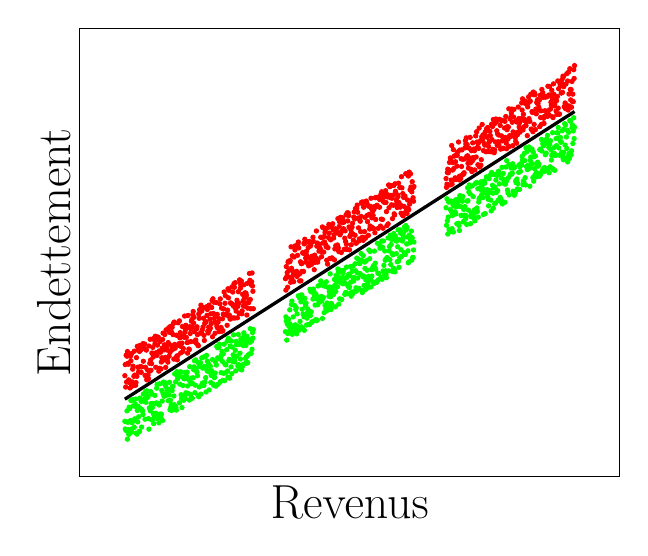
\begin{tikzpicture}


\begin{axis}[xtick=\empty, ytick=\empty, xlabel={\LARGE Revenus}, ylabel={\LARGE Endettement}]
\myGlobalTransformation{0}{0};

% pauvres
\addplot [green, only marks, mark=*, samples=300, mark size=0.75,domain=-3:1]{rand+x};
\addplot [red, only marks, mark=*, samples=300, mark size=0.75,domain=-3:1]{rand+x+2.5};

%moyens
\addplot [green, only marks, mark=*, samples=300, mark size=0.75,domain=2:6]{rand+x};
\addplot [red, only marks, mark=*, samples=300, mark size=0.75,domain=2:6]{rand+x+2.5};

%riches
\addplot [green, only marks, mark=*, samples=300, mark size=0.75,domain=7:11]{rand+x};
\addplot [red, only marks, mark=*, samples=300, mark size=0.75,domain=7:11]{rand+x+2.5};

%frontière
\addplot [black, very thick, domain=-3:11] {x+1.25};
\end{axis}


\end{tikzpicture}
\caption{\label{fig:xdiff} Multi-modal wages and indebtedness data generating mechanism with $y = \{0,1\}$ classes displayed in \textcolor{red}{red} and \textcolor{green}{green} respectively.}
\end{figure}

The second failing situation is the counterpart of the first tailored data generating mechanism. This time, suppose the covariates wages and indebtedness are uniformly sampled. Suppose there is a third categorical feature ``wages source'' which is drawn uniformly from three levels: renters, salaried workers and self-employed. One could argue that renters' risk level do not depend on their indebtedness, which is typically low (and a higher one is a major red flag), salaried workers' risk level is positively correlated with their indebtedness ratio as was the case for the first introductory example (see Figure~\ref{fig:xdiff}) and self-employed people's risk level is negatively correlated with this indebtedness ratio (say, the higher their personal engagement, the higher the chances of success of their business). This example data generating mechanism is illustrated on Figure~\ref{fig:ydiff}. In this situation, and contrary to the first example, an unsupervised generative clustering algorithm like \gls{pca} would not partition the data and the \textit{Credit Scoring} practitioner would construct only one scorecard. This scorecard would have high model bias since it is too simple to accommodate for the variety of the data generating mechanism and consequently perform poorly. This particular data generating mechanism is also revisited in the Experiments of Section~\ref{subsec:num_sim}.


\begin{figure}
\centering
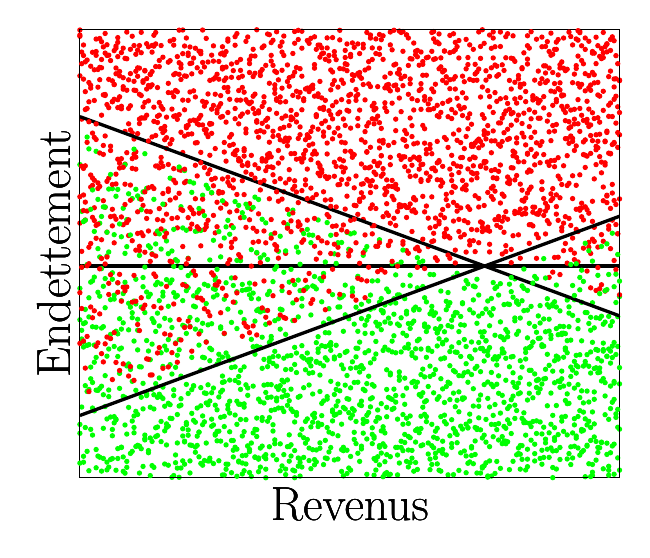
\begin{tikzpicture}


\begin{axis}[xtick=\empty, ytick=\empty, xlabel={\LARGE Revenus}, ylabel={\LARGE Endettement},domain=-3:1, enlargelimits=false,ymin=-3,ymax=6]
\myGlobalTransformationbis{0}{0};

% techniciens
\addplot [green, only marks, mark=*, samples=300, mark size=0.75,domain=-3:1]{rand};
\addplot [green, only marks, mark=*, samples=300, mark size=0.75,domain=-3:1]{rand-2};
\addplot [green, only marks, mark=*, samples=300, mark size=0.75,domain=-3:1]{rand-4};
\addplot [red, only marks, mark=*, samples=300, mark size=0.75,domain=-3:1]{rand+2.5};
\addplot [red, only marks, mark=*, samples=300, mark size=0.75,domain=-3:1]{rand+4.5};
\addplot [red, only marks, mark=*, samples=300, mark size=0.75,domain=-3:1]{rand+6.5};

%frontière
\addplot [black, very thick, domain=-3:1] {1.25};
\end{axis}





\begin{axis}[xtick=\empty, ytick=\empty, xlabel={\LARGE Revenus}, ylabel={\LARGE Endettement},domain=-3:1, enlargelimits=false,ymin=-3,ymax=6]
\myGlobalTransformationbis{0}{3};

% cadres
\addplot [green, only marks, mark=*, samples=300, mark size=0.75,domain=-3:1]{rand-x};
\addplot [green, only marks, mark=*, samples=300, mark size=0.75,domain=-3:1]{rand-x-2};
\addplot [green, only marks, mark=*, samples=300, mark size=0.75,domain=-3:1]{rand-x-4};
\addplot [red, only marks, mark=*, samples=300, mark size=0.75,domain=-3:1]{rand-x+2.5};
\addplot [red, only marks, mark=*, samples=300, mark size=0.75,domain=-3:1]{rand-x+4.5};
\addplot [red, only marks, mark=*, samples=300, mark size=0.75,domain=-3:1]{rand-x+6.5};

%frontière
\addplot [black, very thick, domain=-3:1] {-x+1.25};
\end{axis}



\begin{axis}[xtick=\empty, ytick=\empty, xlabel={\LARGE Revenus}, ylabel={\LARGE Endettement},domain=-3:1, enlargelimits=false,ymin=-3,ymax=6]
\myGlobalTransformationbis{0}{6};

% libérales
\addplot [green, only marks, mark=*, samples=300, mark size=0.75,domain=-3:1]{rand+x};
\addplot [green, only marks, mark=*, samples=300, mark size=0.75,domain=-3:1]{rand+x-2};
\addplot [green, only marks, mark=*, samples=300, mark size=0.75,domain=-3:1]{rand+x-4};
\addplot [red, only marks, mark=*, samples=300, mark size=0.75,domain=-3:1]{rand+x+2.5};
\addplot [red, only marks, mark=*, samples=300, mark size=0.75,domain=-3:1]{rand+x+4.5};
\addplot [red, only marks, mark=*, samples=300, mark size=0.75,domain=-3:1]{rand+x+6.5};
\addplot [red, only marks, mark=*, samples=300, mark size=0.75,domain=-3:1]{rand+x+8.5};

%frontière
\addplot [black, very thick, domain=-3:1] {x+1.25};
\end{axis}



\end{tikzpicture}
\caption{\label{fig:ydiff} Uni-modal wages and indebtedness data generating mechanism with $y = \{0,1\}$ classes displayed in \textcolor{red}{red} and \textcolor{green}{green} respectively which depends on a third feature.}
\end{figure}








\section{Literature review} \label{sec:literature}

This Section aims at providing an eluded literature review of some well-known supervised clustering approaches that could be transposed to the \textit{Credit Scoring} industry.

\subsection{Clustering methods}

In the preceding Section, examples of classical unsupervised clustering methods were given: \gls{pca} (continuous data), \gls{mca} (categorical data) and ultimately \gls{famd} (mixed data). In this Section, focus is given to supervised generative methods. Indeed, a fully generative model $p(\glssymbol{bx},y)$, if sufficiently flexible, could have easily spotted the bottlenecks of the failures of the \gls{pca} approach illustrated on Figures~\ref{fig:xdiff} and~\ref{fig:ydiff}.

\paragraph{\gls{pls}}

~\cite{wold1984collinearity}. The \gls{pls} algorithm seeks to combine the strengths, in its original proposal, of \gls{pca} in explaining the variance of the features $\glssymbol{bx}$ and regression in predicting $y$ with the resulting principal components. In a classification setting, it is termed PLS-DA where DA stands for discriminant analysis.

The .


\paragraph{\gls{spc}}

~\cite{bair2006prediction}. It is motivated by genomics applications where $d > n$ but is applicable to our current setting as well, and by the fact that, in a predictive setting, variance of the features $\glssymbol{bx}$ is only interesting of correlated with $y$. The inner-workings of the algorithm are relatively simple: the correlation between each feature $x_j$ and $y$ is computed. Only the features for which this correlation exceeds a user-defined threshold are retained, and the first few principal components of these features are calculated and used to predict $y$.

There is a close link between \gls{pls} and \gls{spc} that is thoroughly explained in~\cite{friedman2001elements} Section .

For numerical experiments of Section~\ref{sec:num_exp}, the \gls{pls} approach will be used.

\subsection{Direct approaches: logistic regression trees}

\paragraph{\gls{lotus}}

The first research work focusing on a similar problem than the present one seems to be \gls{lotus}~\cite{chan2004lotus}, where logistic regression trees are constructed so as to select features to split the data into sub-populations which break the linearity assumption of \gls{lr} and with an application case similar to ours, namely the insurance market.

Their motivation is that \gls{lr} has a fixed parameter space, defined by the number of input features, whereas trees adapt their flexibility (\textit{i.e.}\ depth) to the sample size $n$; however, trees perform well for classification (\textit{i.e.}\ by setting $\hat{y} = \argmax_y p(y | \glssymbol{bx})$ they can achieve low classification error) but poorly in assessing the probability of the event (\textit{i.e.}\ the estimate of $p(y\glssymbol{bx})$ is the proportion of the event $y$ among observations $\glssymbol{bx}$ at each leaf) as it is piecewise constant; if the true decision boundary separating the two classes of $y$ given $\glssymbol{bx}$ is linear, they need an infinite depth to estimate it as well as \gls{lr}. Thus, they search for trees which leaves are \gls{lr} with few, continuous only, features and which intermediate nodes split the population based on categorical or continuous features which relationship to the log-odd ratio of $y$ is not linear (\textit{i.e.}\ features that would perform poorly in a \gls{lr}).

They propose a feature selection method for node splits that is bias-free: as seen in Chapters~\ref{chap4} and~\ref{chap5}, the number of partitions of $l_j$ labelled factor levels into $m_j$ unlabelled categories (which would here be the tree split criterion) is huge which yields overfitting; thus, their approach relies on a $\chi^2$ test which degrees of freedom is linked to the number of potential rearrangements of $l_j$ into 2 bins. Their optimized criterion is the sum of the log-likelihoods of the \gls{lr} on the tree's leaves. Of course, this leads also to overfitting which requires the tree to be pruned (as is classical for classification trees) using a method closely related to the one developed in the classical CART~\cite{cart84} algorithm. Lastly, their proposed method is not directly applicable to missing values: these observations are not used during training (in the \textit{Credit Scoring} industry, there would most likely be at least one missing value for each observation) and during test, their missing values are imputed by the mean or median.

To sum up, although their intent is similar to ours, \gls{lotus} is not directly usable since only continuous features are used as predictive features in the \gls{lr} of the tree's leaves, it does not handle missing values gracefully, and there are currently no implementation available in \textsf{R} or Python.

\paragraph{\gls{lmt}}

The second approach very close to our industrial problem is named \gls{lmt}~\cite{landwehr2005logistic}. As for~\gls{lotus}, the result is a tree of \gls{lr} at its leaves and the motivation is very similar. Their introductory example, reproduced here with permission on Figure~\ref{fig:lmt} is enlightening: a quadratic boundary cannot be well approximated by trees or \gls{lr} alone, but a combination of both achieves good performance and interpretation.

Their approach differs however drastically from~ \gls{lotus} in that they rely on a particular boosting approach derived from the LogitBoost algorithm~\cite{friedman2000additive} to adjust the \gls{lr} and the classical C4.5 algorithm to grow the tree. The two central ideas behind their usage of the LogitBoost algorithm are simple: it allows to have a stagewise-like process where one feature enters the model at each step and to ``refine'' recursively the \gls{lr} by boosting the \gls{lr} fitted at a node's parent. This most probably induces less parameter estimation variance in each leaves since they partly benefit from samples not in their leaves but used to fit the parents' \gls{lr}. One if its main advantages compared to other approaches is that it is fast. Here again, the resulting tree must be pruned and a tactic similar to CART~\cite{cart84} is used.

However, categorical features are dummy / one-hot encoded so that only a few factor levels might be selected at each leaf, which amount to merging the not selected levels into a reference value. Conversely, when used as a split feature, each level yields a distinct branch. Moreover, missing values are imputed by the mean or mode.

Its original implementation is in Weka but \textsf{R} packages \rinline{party} and \rinline{partykit} provide interfaces and wrappers to it.

\paragraph{\gls{mob}}

Lastly, a third approach closely related to our problem is \gls{mob}~\cite{zeileis2008model} which is an adaptation of a better-known paper~\cite{hothorn2006unbiased} to parametric models in the leaves of a recursively partitioned dataset (hence the name).

Their algorithm consists in fitting the chosen model (in our case, \gls{lr}) for all observations $(\glssymbol{bbx},\glssymbol{bby})$ at the current node and decide to split these into subsets based on a correlation measure of the residuals of the current model and splitting features $V_1, \dots, V_p$ which are not included in $\glssymbol{bbx}$. The procedure is repeated until no significant ``correlation'' is detected. Similarly to \gls{lotus} and contrary to the C4.5 algorithm, which for categorical features and a binary outcome order their levels by their proportion of events $y$ and split as if the feature were ordinal (it can be shown that it is optimal, see~\cite{friedman2001elements} Section 9.2.4), splitting with categorical features require $2^{l_j}$ tests for binary splits. Moreover, there is no mention to eventual treatment of missing values. The number of segments per split is searched exhaustively.

Its implementation is available through the \textsf{R} packages \rinline{party} and \rinline{partykit}.

In the next Section, the problem is formalized as a model selection problem, similarly to the three approaches presented here, with our own notations introduced in the previous Section and Chapters.


\section{Logistic regression trees as a combinatorial model selection problem} \label{sec:model_selec_tree}


\subsection{Cardinality example}


\subsection{Logistic regression tree selection}

Forme de l'arbre en proba ?

\[ \forall \glssymbol{bx}, y, \exists c^\star \in \glssymbol{N}_{K^\star}, \glssymbol{bth}^{\star,c^\star}, p(y | \glssymbol{bx}) = p_{\glssymbol{bth}^{\star,c^\star}}(y | \glssymbol{bx}, c^\star) \]

For $c \in \glssymbol{N}_{K^\star}$, I denote by $(\glssymbol{bbx}^c, \glssymbol{bby}^c)$ the subset of observations of $(\glssymbol{bbx}, \glssymbol{bby})$ for which $c^\star = c$.

The above mentioned \gls{lotus}, \gls{lmt} and \gls{mob}

\begin{align*}
p(\glssymbol{bby}, \glssymbol{bbx}) & =  \sum_{c=1}^{K^\star} p(\glssymbol{bby} | \glssymbol{bbx}, c) p(c | \glssymbol{bbx}) p(\glssymbol{bbx}) & \text{(only $c = c^\star$ is non-zero)} \\
 & = \prod_{c=1}^{K^\star} p(\glssymbol{bby}^c | \glssymbol{bbx}^c, c) p(\glssymbol{bbx}) \\
 & = \prod_{c=1}^{K^\star} \int_{\Theta_c} p_{\glssymbol{bth}^{c}}(\glssymbol{bby}^c | \glssymbol{bbx}^c, c) p(\glssymbol{bth}^c) d\glssymbol{bth}^c p(\glssymbol{bbx}) \\
\ln p(\glssymbol{bby}, \glssymbol{bbx}) & = \sum_{c=1}^{K^\star} \exp \left( \frac{-\text{BIC}(\hat{\glssymbol{bth}^c}) + O(1)}{2} \right) + \ln p(\glssymbol{bbx})
\end{align*}




\begin{equation} \label{eq:BICc}
(K^\star, c^\star) = \argmin_{K,c} \sum_{c=1}^{K} \text{BIC}(\hat{\glssymbol{bth}}^c)
\end{equation}


In the next Section, a relaxation of the constraint of Equation~\eqref{eq:def_c} is proposed, exactly as was done for quantizations in Chapter~\ref{chap4}, by using a continuous approximation of this discrete (and thus highly difficult to directly optimize) problem.


\section{A mixture and latent feature-based relaxation}

\begin{align*}
p(y | \glssymbol{bx}) & = \sum_{c = 1}^K p(y | \glssymbol{bx}, c) p(c | \glssymbol{bx})
\end{align*}


\begin{align*}
p(c | \glssymbol{bx}, y) & \appropto p_{\glssymbol{bth}^c}(y | \glssymbol{bx}, c) p(c | \glssymbol{bx})
\end{align*}


\section{A stochastic estimation strategy}




\section{Extension to quantization and interactions}



\section{Numerical experiments} \label{sec:num_exp}



\subsection{Empirical consistency on simulated data} \label{subsec:num_sim}


\begin{enumerate}[(a)]
\item 
\item 
\end{enumerate}

\subsection{Benchmark on \textit{Credit Scoring} data}




\bigskip

This chapter was .


\printbibliography[heading=subbibliography, title=References of Chapter 5]

